\documentclass[11pt,a4paper]{article}
\usepackage{amsmath,amsthm,amsfonts,amssymb,amscd}
\usepackage{enumerate} 
\usepackage{physics}
\usepackage{enumerate}
\usepackage{fancyhdr}
\usepackage{hyperref}
\usepackage{graphicx}
\hypersetup{colorlinks,
    linkcolor=blue,
    citecolor=blue,      
    urlcolor=blue
}
\usepackage{xurl}

\oddsidemargin0.1cm 
\evensidemargin0.8cm
\textheight22.7cm 
\textwidth15cm \topmargin-0.5cm

\newtheorem{theorem}{Theorem}
\newtheorem{corollary}{Corollary}
\newtheorem{lemma}{Lemma}
\newtheorem{proposition}{Proposition}

\theoremstyle{definition}
\newtheorem{remark}{Remark}
\newtheorem{definition}{Definition}
\newtheorem{observation}{Observation}
\newtheorem{note}{Note}
\newtheorem{hope}{Hope}
\newtheorem{warning}{Warning}
\newtheorem{problem}{Problem}
\newtheorem{fear}{Fear}
\newtheorem{question}{Question}

\newcommand{\Z}{\mathbb{Z}}
\newcommand{\R}{\mathbb{R}}
\newcommand{\C}{\mathbb{C}}
\newcommand{\Q}{\mathbb{Q}}
\newcommand{\A}{\mathbb{A}}

\usepackage{listings}
\usepackage{xcolor}

\definecolor{codegreen}{rgb}{0,0.6,0}
\definecolor{codegray}{rgb}{0.5,0.5,0.5}
\definecolor{codepurple}{rgb}{0.58,0,0.82}
\definecolor{backcolour}{rgb}{0.95,0.95,0.92}

\lstdefinestyle{mystyle}{
    backgroundcolor=\color{backcolour},   
    commentstyle=\color{codegreen},
    keywordstyle=\color{magenta},
    numberstyle=\tiny\color{codegray},
    stringstyle=\color{codepurple},
    basicstyle=\ttfamily\footnotesize,
    breakatwhitespace=false,         
    breaklines=true,                 
    captionpos=b,                    
    keepspaces=true,                 
    numbers=left,                    
    numbersep=5pt,                  
    showspaces=false,                
    showstringspaces=false,
    showtabs=false,                  
    tabsize=2
}

\lstset{style=mystyle}

\newcommand{\MultiSet}{\mathrm{MultiSet}}
\newcommand{\len}{\mathrm{len}}
\newcommand{\din}{\texttt{d\_in}}
\newcommand{\dout}{\texttt{d\_out}}
\newcommand{\T}{\texttt{T} }
\newcommand{\Relation}{\texttt{relation}}
\newcommand{\X}{\mathcal{X}}
\newcommand{\Y}{\mathcal{Y}}
\newcommand{\True}{\texttt{True}}
\newcommand{\False}{\texttt{False}}
\newcommand{\clamp}{\texttt{clamp}}
\newcommand{\function}{\texttt{function}}
\newcommand{\float}{\texttt{float }}
\newcommand{\questionc}[1]{\textcolor{red}{\textbf{Question:} #1}}

\newcommand{\silvia}[1]{{ {\color{blue}{(silvia)~#1}}}}
\newcommand{\grace}[1]{{ {\color{purple}{(grace)~#1}}}}
\newcommand{\connor}[1]{{ {\color{teal}{(connor)~#1}}}}
\newcommand{\mike}[1]{{ {\color{green}{(mike)~#1}}}}
\newcommand{\todo}{{\textcolor{red}{TODO }}}


\title{Privacy Proofs for OpenDP: Clamping}
\author{S\'ilvia Casacuberta}
\date{Summer 2021}

\begin{document}

\maketitle

\tableofcontents

%\section{Remaining Gaps between Proof and Code}
%The proof in this document is being given assuming that the Rust code implements the trait \texttt{TotalOrd}. This is still not the case in the library, where the weaker (and insufficient for this proof) condition of \texttt{PartialOrd} is required. Hence, the Rust code in the OpenDP library is not quite correct in its current state.\footnote{As of August 9, 2021.}

\section{Versions of definitions documents}
\label{sec:versioned-docs}

When looking for definitions for terms that appear in this document, the following versions of the definitions documents should be used.

\begin{itemize}
    \item \textbf{Pseudocode definitions document:} This proof file uses the version of the pseudocode definitions document available as of September 6, 2021, which can be found at \href{https://github.com/opendp/whitepapers/blob/f8b279ab249934182f306138fa14e6390ddae3e9/pseudocode-defns/pseudocode_defns.pdf}{this link} (archived \href{https://web.archive.org/web/20210906201546/https://raw.githubusercontent.com/opendp/whitepapers/pseudocode-defns/pseudocode-defns/pseudocode_defns.pdf}{here}).
    
    \item \textbf{Proof definitions document:} This file uses the version of the proof definitions document available as of September 6, 2021, which can be found at \href{https://github.com/opendp/whitepapers/blob/d4c24e55cc37878634fec0b7f5c89259a3ad3ded/proof-defns/proof_defns.pdf}{this link} (archived \href{https://web.archive.org/web/20210906201056/https://raw.githubusercontent.com/opendp/whitepapers/proof-defns/proof-defns/proof_defns.pdf}{here}). 
\end{itemize}

\section{Algorithm implementation}

\subsection{Code in Rust}
The current OpenDP library contains the \texttt{make\_clamp\_vec} function implementing the clamping function. This is defined in lines 25-38 of the file \texttt{manipulation.rs} in the Git repository\footnote{As of June 16, 2021. Since then, the trait \texttt{PartialOrd} has been updated to \texttt{TotalOrd}.}  (\url{https://github.com/opendp/opendp/blob/58feb788ec78ce739caaf3cad8471c79fd5e7132/rust/opendp/src/trans/manipulation.rs#L25-L38}).

\begin{figure}[ht]
    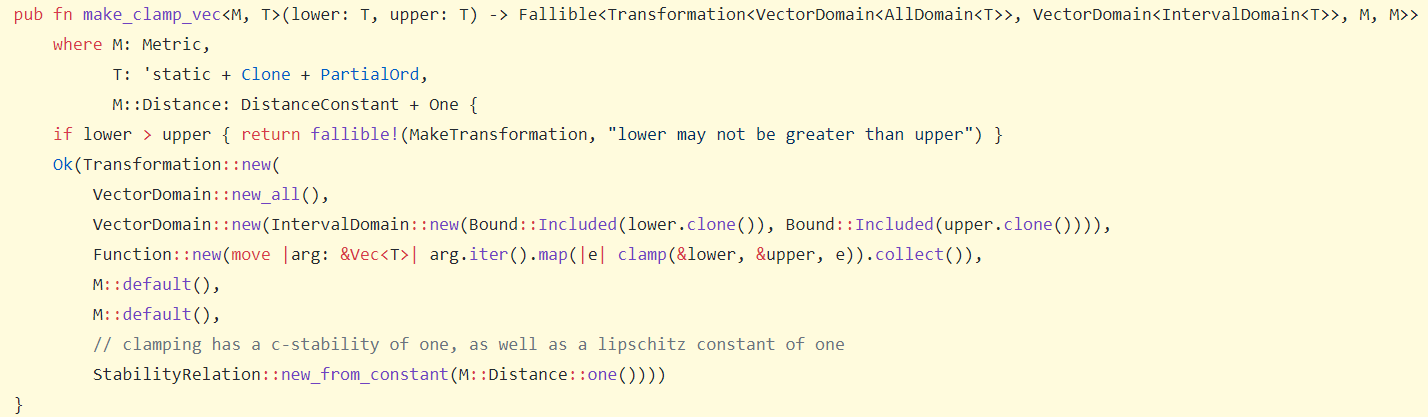
\includegraphics[width=16cm]{clamp_rust.png}
    \centering
    \label{fig:code}
\end{figure}

%Since then, the code has been updated to include a more general clampable domain to abstract together parts of the vector and scalar cases:\footnote{As of July 28, 2021.} \url{https://github.com/opendp/opendp/blob/main/rust/opendp/src/trans/clamp.rs#L28-L44} in conjunction with \url{https://github.com/opendp/opendp/blob/main/rust/opendp/src/trans/clamp.rs#L74-L85}. We decided not to refer to the clampable domain in the proofs given that we are separating the vector and scalar cases into two different proof documents.

%\begin{figure}[ht]
 %   \includegraphics[width=16cm]{clamp3.png}
 %   \centering
 %   \label{fig:code}
%\end{figure}

%\begin{figure}[ht]
 %   \includegraphics[width=16cm]{clamp4.png}
 %   \centering
 %   \label{fig:code}
%\end{figure}

\subsection{Pseudocode in Python}\label{sec:pseudocode}
We present a simplified Python-like pseudocode of the Rust implementation below. The necessary definitions for the pseudocode can be found at \href{https://www.overleaf.com/project/60d215bf90b337ac02200a99}{``List of definitions used in the pseudocode"}. 

\emph{The use of \texttt{code}-style parameters in the preconditions section below (for example, \texttt{input\_domain}) means that this information should be passed along to the \texttt{Transformation} constructor.}

\subsubsection*{Preconditions}
To ensure the correctness of the output, we require the following preconditions:

\begin{itemize}
    \item \textbf{User-specified types:}
    \begin{itemize}
        \item Type \texttt{T} must have trait \texttt{TotalOrd}.
    \end{itemize}
\end{itemize}

\subsubsection*{Postconditions}
\begin{itemize}
    \item Either a valid \texttt{Transformation} is returned or an error is returned.
\end{itemize}

\begin{lstlisting}[language=Python, escapechar=|] 
def MakeClamp(L: T, U: T): |\label{line:def}|
    input_domain = VectorDomain(AllDomain(T))
    output_domain = VectorDomain(IntervalDomain(L, U)) |\label{line:output}|
    input_metric = SymmetricDistance()
    output_metric = SymmetricDistance()
    
    def relation(d_in: u32, d_out: u32) -> bool: |\label{line:rel}|
        return d_out >= d_in*1
    
    def function(data: Vec[T]) -> Vec[T]: |\label{line:fn}|
        def clamp(x: T) -> T: |\label{line:clamp}|
            return max(min(x, U), L)
        return list(map(clamp, data)) |\label{line:map}|
    
    return Transformation(input_domain, output_domain, function, input_metric, output_metric, stability_relation = relation)
\end{lstlisting}


\section{Proof}
The necessary definitions for the proof can be found at \href{https://www.overleaf.com/project/60d214e390b337703d200982}{``List of definitions used in the proofs"}.

\subsection{Symmetric distance}
\begin{theorem}
    For every setting of the input parameters \texttt{(L, U)} to \texttt{MakeClamp} such that the given preconditions
    hold, \texttt{MakeClamp} raises an exception (at compile time or run time) or returns a valid transformation with the following properties:
    \begin{enumerate}
        \item \textup{(Appropriate output domain).} For every element $v$ in \texttt{input\_domain}, $\function(v)$ is in \texttt{output\_domain}. % Prof. Vadhan said on 29/6 to leave it as this for now, but maybe in the future we add to the theorem statement what exactly the input domain and output domain are (although of course we already say this in the proof)
        
        \item \textup{(Domain-metric compatibility).} The domain \texttt{input\_domain} matches one of the possible domains listed in the definition of \texttt{input\_metric}, and likewise \texttt{output\_domain} matches one of the possible domains listed in the definition of \texttt{output\_metric}.
        
        \item \textup{(Stability guarantee).} For every pair of elements $v, w$ in \texttt{input\_domain} and for every pair $(\din, \dout)$, where $\din$ has the associated type for \texttt{input\_metric} and $\dout$ has the associated type for \texttt{output\_metric}, if $v,w$ are $\din$-close under \texttt{input\_metric} and $\Relation(\din, \dout) = \True$, then $\function(v), \function(w)$ are $\dout$-close under \texttt{output\_metric}.
    \end{enumerate}
\end{theorem}

\begin{proof}
\textbf{(Appropriate output domain).} In the case of \texttt{MakeClamp}, this corresponds to showing that for every vector $v$ of elements of type \texttt{T}, $\function(v)$ is a vector of elements of type \texttt{T} which are contained in the interval \texttt{[L, U]}. For that, we need to show two things: first, that \texttt{function(v)} has type \texttt{Vec[T]}.
Second, that they belong to the interval \texttt{[L, U]}.

Firstly, that $\function(v)$ has type \texttt{Vec[T]} follows from the assumption that element $v$ is in \texttt{input\_domain} and from the type signature of \texttt{function} in line~\ref{line:fn} of the pseudocode (Section~\ref{sec:pseudocode}), which takes in an element of type \texttt{Vec[T]} and returns an element of type \texttt{Vec[T]}. If the Rust code compiles correctly, then the type correctness follows from the definition of the type signature enforced by Rust. Otherwise, the code raises an exception for incorrect input type. 

Secondly, we need to show that the vector entries belong to the interval \texttt{[L, U]}. For that, it is foremost necessary that \texttt{L} $\leq$ \texttt{U}. This condition is already checked when declaring \texttt{output\_domain = VectorDomain(IntervalDomain(L, U))} in line~\ref{line:output} of the pseudocode. This check already exists via the construction of \texttt{IntervalDomain}, which returns an error if \texttt{L} $>$ \texttt{U}. The rest follows from the definition of \texttt{clamp} in line \ref{line:clamp}. According to line \ref{line:clamp} in the pseudocode, there are 3 possible cases to consider:
\begin{enumerate}
    \item \texttt{x} $>$ \texttt{U}: then $\clamp\texttt{(x)}$ returns \texttt{U}.
    \item \texttt{x} $\in$ \texttt{[L, U]}: then $\clamp\texttt{(x)}$ returns \texttt{x}.
    \item \texttt{x} $<$ \texttt{L}: then $\clamp\texttt{(x)}$ returns \texttt{L}.
\end{enumerate}
In all three cases, the returned value of type \T is contained in the interval \texttt{[L, U]}. Hence, the vector $\function(v)$ returned in line~\ref{line:map} of the pseudocode is an element of \texttt{output\_domain}.

Lastly, both \texttt{L} and \texttt{U} have type \texttt{T} by the type signature of \texttt{MakeClamp}. Both the definition of \texttt{IntervalDomain} and that of the \texttt{clamp} function (line~\ref{line:clamp} in the pseudocode, which uses the \texttt{min} and \texttt{max} functions) require that \texttt{T} implements \texttt{TotalOrd}, which holds by the preconditions.

\smallskip
\textbf{(Domain-metric compatibility).} For \texttt{MakeClamp}, both the input and output cases correspond to showing that \texttt{VectorDomain(T)} is compatible with the symmetric distance metric. This follows directly from the definition of symmetric distance, as stated in \href{https://www.overleaf.com/project/60d215bf90b337ac02200a99}{``List of definitions used in the pseudocode"}.

\smallskip
\textbf{(Stability guarantee).} Throughout the stability guarantee proof, we can assume that $\function(v)$ and $\function(w)$ are in the correct output domain, by the \textit{appropriate output domain property} shown above. 

Since by assumption $\Relation(\din, \dout) = \True$, by the \texttt{MakeClamp} stability relation (as defined in line~\ref{line:rel} in the pseudocode), we have that $\din \leq \dout$. Moreover, $v, w$ are assumed to be $\din$-close. By the definition of the symmetric difference metric, this is equivalent to stating that $d_{Sym}(v, w) = |\MultiSet(v) \Delta \MultiSet(w)| \leq \din$.

Let $\mathcal{X}$ be the domain of all elements of type \texttt{T}. By applying the histogram notation,\footnote{Note that there is a bijection between multisets and histograms, which is why the proof can be carried out with either notion. For further details, please consult \url{https://www.overleaf.com/project/60d214e390b337703d200982}.}  it follows that
\[
d_{Sym}(v, w) = \lVert h_{v} - h_{w}\rVert_1 = \sum_{z \in \mathcal{X}} |h_v(z) - h_w(z)| \leq \din \leq \dout.
\]

By Definition 3.10 in \href{https://www.overleaf.com/project/60d214e390b337703d200982}{``List of definitions used in the proofs"} and the definition of \texttt{clamp} in lines \ref{line:clamp}--\ref{line:map} in the pseudocode, it follows that the \texttt{function} defined in \texttt{MakeClamp}, which maps elements from \texttt{VectorDomain} to \texttt{VectorDomain}, is a row transform. Therefore, by Lemma 3.13 in \href{https://www.overleaf.com/project/60d214e390b337703d200982}{``List of definitions used in the proofs"}, it follows that for every pair of elements $v, w$ in \texttt{input\_domain},
\[
    d_{Sym}(\texttt{function}(v), \texttt{function}(w)) \leq d_{Sym}(v, w).
\]
Then, by the initial assumptions \texttt{relation(\din, \dout) = True} and $\din \leq \dout$, it follows that
\[
    d_{Sym}(\texttt{function}(v), \texttt{function}(w)) \leq d_{Sym}(v, w) \leq \din \leq \dout.
\]
Hence,
\[
    d_{Sym}(\texttt{function}(v), \texttt{function}(w)) \leq \dout,
\]
as we wanted to show.
\end{proof}

\newpage

\section{Old proof for the stability guarantee}
Salil suggested introducing the definition of row transform and adding a general lemma for its stability guarantee, as shown in Section 3.3 in \href{https://www.overleaf.com/project/60d214e390b337703d200982}{``List of definitions used in the proofs"}. However, we keep the longer old proof (case-by-case) for completeness, and in case any issues arise when revising the definition and theorems relating to row transforms

\begin{proof}
\smallskip
\textbf{(Stability guarantee).} Throughout the stability guarantee proof, we can assume that $\function(v)$ and $\function(w)$ are in the correct output domain, by the \textit{appropriate output domain property} shown above. 

Since by assumption $\Relation(\din, \dout) = \True$, by the \texttt{MakeClamp} stability relation (as defined in line~\ref{line:rel} in the pseudocode), we have that $\din \leq \dout$. Moreover, $v, w$ are assumed to be $\din$-close. By the definition of the symmetric difference metric, this is equivalent to stating that $d_{Sym}(v, w) = |\MultiSet(v) \Delta \MultiSet(w)| \leq \din$.

Let $\mathcal{X}$ be the domain of all elements of type \texttt{T}. By applying the histogram notation,\footnote{Note that there is a bijection between multisets and histograms, which is why the proof can be carried out with either notion. For further details, please consult \url{https://www.overleaf.com/project/60d214e390b337703d200982}.}  it follows that
\[
d_{Sym}(v, w) = \lVert h_{v} - h_{w}\rVert_1 = \sum_{z \in \mathcal{X}} |h_v(z) - h_w(z)| \leq \din \leq \dout.
\]

We now consider $\MultiSet(\function(v))$ and $\MultiSet(\function(w))$.
For each element $z \in \MultiSet(v) \cup \MultiSet(w)$, where $z$ has type \texttt{T}, if $z \in \MultiSet(v) \Delta \MultiSet(w)$, we will assume wlog that $z \in \MultiSet(v) \setminus \MultiSet(w)$. We consider the following cases:

\begin{enumerate}
    \item $z >$ \texttt{U} or $z <$ \texttt{L}: then, in the former case, $\clamp(z) =$ \texttt{U}. First consider the case when $z \in \MultiSet(v) \cup \MultiSet(w)$ with the same multiplicity in both multisets. Then, $|h_{\function(v)}(z) - h_{\function(w)}(z)| = 0$ because we have both $h_{\function(v)}(z) = 0$ and $h_{\function(w)}(z) = 0$. Thus the sum
    \[
    \sum_{z \in \mathcal{X}} |h_{\function(v)}(z) - h_{\function(w)}(z)|
    \]
    remains invariant, because the quantity $|h_{v}(z) - h_{w}(z)|$ is added to $|h_{\function(v)}(\texttt{U}) - h_{\function(w)}(\texttt{U})|$, given that $\clamp(z) = \texttt{U}$. 
    
    Suppose $z$ has multiplicity $k_v \geq 0$ in $\MultiSet(v)$ and multiplicity $k_w \geq 0$ in $\MultiSet(w)$, where $k_v \neq k_w$. After considering $z$, the value $h_{\function(v)}(\texttt{U})$ becomes $h_{\function(v)}(\texttt{U}) + k_v$, and $h_{\function(w)}(\texttt{U})$ becomes $h_{\function(w)}(\texttt{U}) + k_w$. Hence the quantity $|h_{\function(v)}(\texttt{U}) - h_{\function(w)}(\texttt{U})|$ increases by at most $|h_v(z) - h_w(z)|$, since, by the triangle inequality,
    \begin{align*}
         & |(h_{\function(v)}(\texttt{U}) + k_v) - (h_{\function(w)}(\texttt{U}) + k_w)| \leq
    \\[0.2cm]
         & \leq |h_{\function(v)}(\texttt{U}) - h_{\function(w)}(\texttt{U})| + |k_v - k_w| =
    \\[0.2cm]
        & = |h_{\function(v)}(\texttt{U}) - h_{\function(w)}(\texttt{U})| + |h_v(z) - h_w(z)|.
    \end{align*}
    The same argument applies whenever $z < \texttt{L}$.\footnote{The first subcase discussed here, i.e., when $k_v = k_w$, is also proven by the triangle inequality expression above, but it seemed clean to separate the case where the total sum remains invariant.}
    
    \item $z \in \texttt{(L, U)}$: then, $\clamp(z) = z$. Since $h_v(z) = h_{\function(v)}(z)$ and $h_v(w) = h_{\function(w)}(z)$, it follows that $|h_v(z) - h_w(z)| = |h_{\function(v)}(z) - h_{\function(w)}(z)|$. Hence the histogram count, i.e., the quantity
     \[
        \sum_{z \in \mathcal{X}} |h_{\function(v)}(z) - h_{\function(w)}(z)|,
    \]
    remains invariant.
    
    \item $z = \texttt{U}$ or $z = \texttt{L}$: in the former case, $\clamp(z) = \texttt{U}$. If $z \in \MultiSet(v) \cup \MultiSet(w)$ with the same multiplicity in both multisets, then the histogram count remains invariant under the addition of element $z$. Otherwise, if $z \in \MultiSet(v) \setminus \MultiSet(w)$, or if $z$ is in their union but with different multiplicity, then element $z$ can increase the quantity $|h_{\function(v)}(\texttt{U}) - h_{\function(w)}(\texttt{U})|$ by at most $|h_v(z)-h_w(z)|$, following the same reasoning with the triangle inequality as in case~2.
    
    The same argument applies whenever $z = \texttt{L}$.
\end{enumerate}

By aggregating the three cases above, we conclude that
\[
\sum_{z \in \mathcal{X}} |h_{\function(v)}(z) - h_{\function(w)}(z)| \leq \sum_{z \in \mathcal{X}} |h_v(z) - h_w(z)|.
\]
By the initial assumptions, we recall that $\din \leq \dout$, and that $v, w$ are $\din$-close. Then,
\[
\sum_{z \in \mathcal{X}} |h_{\function(v)}(z) - h_{\function(w)}(z)| \leq \sum_{z \in \mathcal{X}} |h_v(z) - h_w(z)| \leq \din \leq \dout.
\]
Therefore, 
\[
|\MultiSet(\function(v)) \Delta \MultiSet(\function(w))| \leq \dout,
\]
as we wanted to show.
\end{proof}

\end{document}
